% IEEE-style paper for the Traffic Violation Detection project.
% Compile with pdflatex (two passes) + bibtex, or upload paper/ to Overleaf.
\documentclass[conference]{IEEEtran}
\usepackage{cite}
\usepackage{amsmath}
\usepackage{graphicx}
\usepackage{booktabs}
\usepackage{tikz}
\usetikzlibrary{positioning}
\usepackage{url}

\title{Event-Level Robustness of Rule-Based Traffic Violation Detection
under Tracker Degradation}
\author{\IEEEauthorblockN{Rakib Islam}
\IEEEauthorblockA{\textit{Department of Computer Science and Engineering}\\
Dhaka, Bangladesh \\
rakibislam4913@gmail.com}}

\begin{document}
\maketitle

\begin{abstract}
Rule-based traffic violation detection pipelines combine an object detector,
a multi-object tracker, per-camera scene calibration, and a rule engine.
A failure mode that is rarely quantified is how \emph{tracker degradation} ---
occlusion, missed detections, and identity switches --- silently destroys
violation events before the rules ever see them. We present a complete,
privacy-preserving pipeline (YOLOv8 detection, ByteTrack tracking, scene
calibration, red-light and wrong-way rules, blurred evidence) together with
two engineering contributions: (i) a constructed-case evaluation methodology
for rare events whose ground truth holds by construction (reversed playback,
synthetic signal overlays), and (ii) a lightweight online tracklet stitcher
with constant-velocity gating. On our constructed real-video event set the
pipeline reaches event-level P/R/F1 of $1.000$; under seeded track dropout,
stitching lifts event recall from $0.333$ to $0.593$ at 30\% dropout and to
$0.963$ at 10\% dropout, with no precision cost. A gate ablation shows the
operating point trades recall against mis-merge risk in dense traffic. All
numbers come from real, seeded runs and are fully reproducible from the
public repository.
\end{abstract}

\section{Introduction}
Traffic violations are rare events buried in hours of footage, and manual
review does not scale. Camera-side systems promise automatic flagging, but
two practical problems are under-reported in student and applied projects.
First, \emph{there is no labeled violation footage}: violations are rare,
camera-specific, and legally sensitive, so standard detection benchmarks do
not answer ``did the rules fire on the right event at the right time?''
Second, rules consume \emph{tracks}, and trackers are fragile: occlusion and
identity switches fragment one vehicle into several tracklets, and a rule
engine that requires sustained observation (e.g.\ opposing motion for $N$
consecutive frames) then produces false negatives that are almost impossible
to notice without an event-level ground truth.

This paper reports a complete pipeline plus an attempt to close those two
gaps. Our contributions are:
\begin{itemize}
  \item a privacy-preserving end-to-end pipeline (detection, tracking,
  scene calibration, rules, evidence, review dashboard) with all evaluation
  artifacts committed and reproducible;
  \item a \emph{constructed-case} event-level evaluation methodology in which
  ground truth holds by construction (reversed playback makes every moving
  vehicle wrong-way; a synthetic signal overlay creates controlled red-light
  scenarios), every label verified by frame-level review --- a methodology
  that caught two real failure modes before any field use;
  \item a lightweight \emph{online tracklet stitcher} (geometry and
  constant-velocity gating, no re-identification model) and a seeded dropout
  study measuring its event-level effect, including a gate ablation that
  exposes the recall / mis-merge trade-off.
\end{itemize}

\section{Related Work}
\textbf{Benchmarks and detection.} UA-DETRAC~\cite{wen2020ua} is the standard
benchmark for vehicle detection and tracking in traffic surveillance. Single-
stage detectors in the YOLO family~\cite{jocher2023yolov8} are the common
choice for real-time surveillance pipelines.

\textbf{Multi-object tracking.} ByteTrack~\cite{zhang2022bytetrack} keeps
every detection box and recovers low-confidence ones, which helps under
occlusion; BoT-SORT~\cite{aharon2022botsort} adds camera-motion compensation
and appearance features. Tracking quality is measured by HOTA~\cite{luiten2021hota},
IDF1~\cite{ristani2016idf1}, and the MOTChallenge suite~\cite{milan2016mot16}.
We deliberately use geometric gating only: our stitcher is complementary to
appearance-based re-ID and cheaper to audit.

\textbf{Event-level evaluation.} Most applied work evaluates detectors (mAP)
or trackers (HOTA/IDF1) but rarely the \emph{violation events} a user actually
cares about. To our knowledge, constructed cases (reversed playback, synthetic
signal overlays) are not a standard published evaluation practice; we report
them as an evaluation methodology alongside the results they produce.

\section{System Design}
Fig.~\ref{fig:arch} shows the pipeline. All behavior is driven by YAML
configs (per-camera scene calibration, tracker, extensions); seeds are fixed
and logged per run.

\begin{figure}[t]
\centering
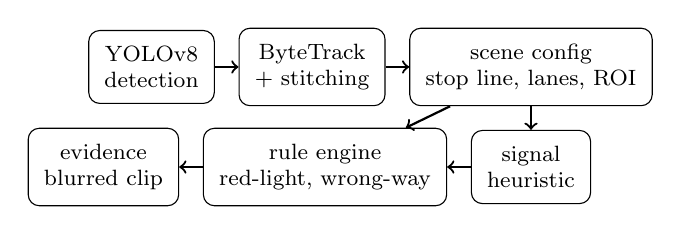
\begin{tikzpicture}[font=\footnotesize,
  box/.style={draw, rounded corners, align=center, minimum height=7mm,
              inner sep=2mm},
  arr/.style={->, thick}]
\node[box] (det) {YOLOv8\\detection};
\node[box, right=3mm of det] (trk) {ByteTrack\\+ stitching};
\node[box, right=3mm of trk] (sce) {scene config\\stop line, lanes, ROI};
\node[box, below=3mm of sce] (sig) {signal\\heuristic};
\node[box, left=3mm of sig] (eng) {rule engine\\red-light, wrong-way};
\node[box, left=3mm of eng] (ev) {evidence\\blurred clip};
\draw[arr] (det) -- (trk);
\draw[arr] (trk) -- (sce);
\draw[arr] (sce) -- (sig);
\draw[arr] (sce) -- (eng);
\draw[arr] (sig) -- (eng);
\draw[arr] (eng) -- (ev);
\end{tikzpicture}
\caption{Pipeline overview. Every box is config-driven; all runs are seeded.}
\label{fig:arch}
\end{figure}

\textbf{Scene and signal.} Each camera is calibrated with a stop-line segment,
lane polygons with expected travel directions, and an optional signal ROI
(cameras without a visible signal disable the red-light rule by config).
Signal state is a color heuristic (HSV vote inside the ROI) with
majority-vote temporal smoothing.

\textbf{Rule engine.} Red-light: a track's ground point crosses the stop line
while the signal is red, past a 0.3\,s grace window; per track, only the
first qualifying crossing fires. Wrong-way: opposing motion versus lane
direction sustained for at least 10 frames. We add a \emph{recross window}:
a crossing onto a side of the stop line the same track already occupied
within the last $5$\,s is suppressed as a bounding-box truncation artifact.
This single change moved event precision on our red-light clip from $0.667$
to $1.000$; the underlying event (a vehicle re-flagged after an occlusion
clears) is analyzed in Sec.~\ref{sec:constructed}.

\textbf{Evidence and privacy.} Each event yields a short clip (default 7\,s),
a blurred keyframe, and JSON metadata, stored in SQLite behind a FastAPI +
Streamlit review dashboard. Plates and faces are blurred in stored evidence
by default.

\section{Constructed Event-Level Evaluation}
\label{sec:constructed}
With no labeled violation footage available, we built three clips from a real
UA-DETRAC sample (frame 642 of MVI\_20012), each labeled by construction and
verified frame by frame:
\begin{itemize}
  \item \emph{negative}: normal traffic, expected to produce zero events
        (false-alarm check);
  \item \emph{wrong-way}: the same clip reversed, so every sustained moving
        vehicle is wrong-way by construction (7 labeled events);
  \item \emph{red-light}: a synthetic signal overlay (green through frame 25,
        red afterwards); two vehicles cross on red, one crosses legally on
        green (2 labeled events).
\end{itemize}
Predicted and expected events are matched greedily one-to-one by type and
frame-window overlap ($\pm 15$ frames tolerance).

The evaluation earned its keep twice. (i) An occlusion artifact: a van whose
bounding box was truncated behind another vehicle re-crossed the stop line
when the occlusion cleared, firing a spurious red-light event; the recross
window suppresses it. (ii) A mislabeled ``identity-switch duplicate'' that
frame-level review revealed to be a genuine second violator: the two tracks
coexist at different depths early in the clip. We corrected the label, not
the metric --- a reminder that event-level ground truth deserves the same
care as model training data.

\section{Tracklet Stitching under Tracker Degradation}
\textbf{Algorithm.} The stitcher wraps the tracker online. A track absent for
$1..G$ frames becomes a \emph{lost tracklet} storing its last ground point
and a median velocity over the last five consecutive-frame displacements. A
new tracklet is stitched to the lost tracklet whose constant-velocity
prediction (over the gap) is nearest, within a distance gate $D$ px, greedy
nearest-first with one-to-one matching per frame; stitched tracklets adopt
the old identity. The rule engine's observation-gap tolerance is set to the
same $G$, so rules see continuity without fabricating intermediate
detections. We deliberately omit appearance features (no re-ID model): the
method is auditable and CPU-cheap, at the cost of a mis-merge risk in dense
same-direction queues.

\textbf{Study protocol.} Seeded \emph{post-hoc track dropout} (random removal
of per-frame track outputs) emulates detector/tracker misses; being applied
after tracking it is strictly harsher than real detector loss, which we state
as a limitation. Bernoulli dropout at $p\in\{0.1,0.2,0.3\}$ and occlusion-like
bursts (lengths 4 and 8 frames, the latter beyond the stitch gate) are
evaluated over 3 seeds on the three-clip event set; the full matrix runs
with stitching off, on at the deployed gates ($G{=}5$, $D{=}50$\,px), and at
two ablation settings ($3/30$ and $10/80$).

\section{Results}
\textbf{Detection.} Vehicle detector on the UA-DETRAC-10K val split (500
images): mAP@0.5 $=0.970$, mAP@0.5:0.95 $=0.841$ (bus 0.973 / car 0.984 /
truck 0.933 / van 0.992). Extension detectors: helmet 0.920, plate 0.974
mAP@0.5. Degradations (mAP@0.5): night 0.947, rain 0.970, glare 0.969.

\textbf{Event level.} On the constructed set: precision $=$ recall $=$ F1
$=1.000$, zero false alerts on the negative clip, 7/7 wrong-way and 2/2
red-light events matched. Rule unit tests: 9/9 synthetic scenarios.

\textbf{Dropout robustness.} Fig.~\ref{fig:dropout} and
Table~\ref{tab:ablation}: stitching roughly doubles recall at every dropout
level while precision stays $1.000$. Burst length beyond the gate is not
bridged, as designed.

\begin{figure}[t]
\centering
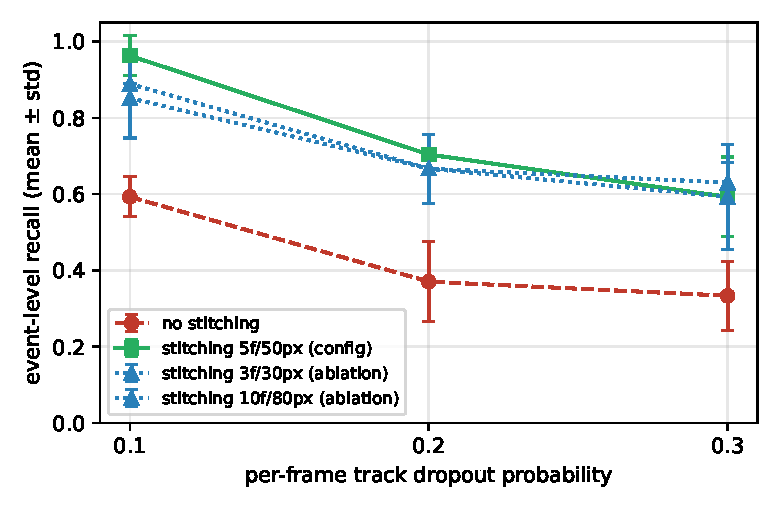
\includegraphics[width=\columnwidth]{figures/dropout_recall.pdf}
\caption{Event-level recall vs.\ seeded track dropout (mean $\pm$ std over 3
seeds). Stitching lifts recall at every level; the deployed mid-range gates
win or tie with both ablation settings --- tighter gates bridge fewer gaps,
looser gates mis-merge nearby vehicles in dense traffic.}
\label{fig:dropout}
\end{figure}

\begin{table}[t]
\centering
\caption{Gate ablation (stitching on; event-level recall, mean $\pm$ std over
3 seeds; bernoulli dropout $p$). Tighter gates bridge fewer gaps; looser
gates mis-merge nearby vehicles in dense queues, so the deployed setting wins
or ties in most cells.}
\label{tab:ablation}
\begin{tabular}{lll}
\toprule
gates (frames/px) & $p{=}0.1$ & $p{=}0.3$ \\
\midrule
no stitching      & 0.593 $\pm$ 0.052 & 0.333 $\pm$ 0.091 \\
deployed (5/50)   & \textbf{0.963} $\pm$ 0.052 & 0.593 $\pm$ 0.105 \\
ablation (3/30)   & 0.889 $\pm$ 0.000 & \textbf{0.630} $\pm$ 0.052 \\
ablation (10/80)  & 0.852 $\pm$ 0.105 & 0.593 $\pm$ 0.139 \\
\bottomrule
\end{tabular}
\end{table}

\section{Limitations}
The event set is three short clips (20.1\,s) --- a smoke test, not field
performance. Dropout is a post-hoc surrogate. Stitching is geometric only;
dense queues can mis-merge (looser gates dropped clean-set recall to $0.778$
during development). Gaps beyond 5 frames are unbridged. The UA-DETRAC
tracking benchmark (HOTA/IDF1) is not run: dataset access is pending.

\section{Ethics and Privacy}
All outputs are candidates for human review; nothing automates penalties.
Plates/faces are blurred by default; evidence clips are short windows, not
continuous footage; raw footage of people is never committed. Deployment
policy recommendations (access control, retention) are in the repository.

\section{Conclusion}
We presented a complete, reproducible traffic-violation pipeline and showed
that the unglamorous parts --- event-level constructed evaluation and tracker
robustness --- are where the real, measurable problems live. The methodology
(transportable to any rare-event detection task) and the stitcher
(double recall under degradation at zero precision cost) are the pieces we
would reuse first.

\bibliographystyle{IEEEtran}
\bibliography{references}

\end{document}
